%%%%%%%%%%%%%%%%%%%%%%%%%%%%%%%%%%%%%%%%%%%%%%%%%%%
%% LaTeX book template                           %%
%% Author:  Amber Jain (http://amberj.devio.us/) %%
%% License: ISC license                          %%
%%%%%%%%%%%%%%%%%%%%%%%%%%%%%%%%%%%%%%%%%%%%%%%%%%%

\documentclass[a4paper,11pt]{book}
\usepackage[a4paper, total={7.5in, 8in}]{geometry}
\usepackage[T1]{fontenc}
\usepackage[utf8]{inputenc}
\usepackage{lmodern}
\usepackage{listings}
\usepackage{alltt}
\usepackage{fancyvrb}
\usepackage[dvipsnames]{xcolor}
%%%%%%%%%%%%%%%%%%%%%%%%%%%%%%%%%%%%%%%%%%%%%%%%%%%%%%%%%
% Source: http://en.wikibooks.org/wiki/LaTeX/Hyperlinks %
%%%%%%%%%%%%%%%%%%%%%%%%%%%%%%%%%%%%%%%%%%%%%%%%%%%%%%%%%
\usepackage{hyperref}
\usepackage{graphicx}
\usepackage[english]{babel}
% \usepackage{IGNrapport,GuideBW,amsmath}
\usepackage{amsmath}
\usepackage{breqn}   % Breaks the equations into linea automatically
\usepackage{amsmath} % Breaks the equations into lines manually putting ``//''
%%%%%%%%%%%%%%%%%%%%%%%%%%%%%%
% Tikz
%%%%%%%%%%%%%%%%%%%%%%%%%%%%%%
\usepackage{tikz}
%%%%%%%%%%%%%%%%%%%%%%%%%%%%%%%%%%%%%%%%%%%%%%%%%%%%%%%%%%%%%%%%%%%%%%%%%%%%%%%%
% 'dedication' environment: To add a dedication paragraph at the start of book %
% Source: http://www.tug.org/pipermail/texhax/2010-June/015184.html            %
%%%%%%%%%%%%%%%%%%%%%%%%%%%%%%%%%%%%%%%%%%%%%%%%%%%%%%%%%%%%%%%%%%%%%%%%%%%%%%%%
\newenvironment{dedication}
{
   \cleardoublepage
   \thispagestyle{empty}
   \vspace*{\stretch{1}}
   \hfill\begin{minipage}[t]{0.66\textwidth}
   \raggedright
}
{
   \end{minipage}
   \vspace*{\stretch{3}}
   \clearpage
}

%%%%%%%%%%%%%%%%%%%%%%%%%%%%%%%%%%%%%%%%%%%%%%%%
% Chapter quote at the start of chapter        %
% Source: http://tex.stackexchange.com/a/53380 %
%%%%%%%%%%%%%%%%%%%%%%%%%%%%%%%%%%%%%%%%%%%%%%%%
\makeatletter
\renewcommand{\@chapapp}{}% Not necessary...
\newenvironment{chapquote}[2][2em]
  {\setlength{\@tempdima}{#1}
   \def\chapquote@author{#2}%
   \parshape 1 \@tempdima \dimexpr\textwidth-2\@tempdima\relax%
   \itshape}
  {\par\normalfont\hfill--\ \chapquote@author\hspace*{\@tempdima}\par\bigskip}
\makeatother

%%%%%%%%%%%%%%%%%%%%%%%%%%%%%%%%%%%%%%%%%%%%%%%%%%%
% First page of book which contains 'stuff' like: %
%  - Book title, subtitle                         %
%  - Book author name                             %
%%%%%%%%%%%%%%%%%%%%%%%%%%%%%%%%%%%%%%%%%%%%%%%%%%%

% Book's title and subtitle
\title{\Huge \textbf{FERMI}\\ \huge Code for nuclear reactor calculations }
% Author
\author{\textsc{Federico Caccia}\\ \textsc{Guido Giuntoli}}

% Images path
\graphicspath{{images/}}

\begin{document}

\frontmatter
\maketitle

%%%%%%%%%%%%%%%%%%%%%%%%%%%%%%%%%%%%%%%%%%%%%%%%%%%%%%%%%%%%%%%
% Add a dedication paragraph to dedicate your book to someone %
%%%%%%%%%%%%%%%%%%%%%%%%%%%%%%%%%%%%%%%%%%%%%%%%%%%%%%%%%%%%%%%

\begin{dedication}
Dedicated to my mum Patricia, dad Miguel, sister Julia and dog Jenny.
\end{dedication}

%%%%%%%%%%%%%%%%%%%%%%%%%%%%%%%%%%%%%%%%%%%%%%%%%%%%%%%%%%%%%%%%%%%%%%%%
% Auto-generated table of contents, list of figures and list of tables %
%%%%%%%%%%%%%%%%%%%%%%%%%%%%%%%%%%%%%%%%%%%%%%%%%%%%%%%%%%%%%%%%%%%%%%%%
\tableofcontents
% \listoffigures
% \listoftables

\mainmatter

%%%%%%%%%%%
% Preface %
%%%%%%%%%%%
% \chapter*{Preface}

\par
After graduating as Nuclear Engineer at Balseiro Institute in Argentina I started thinking in applying what I learned during my final year project on a code for simulating a nuclear reactor by state-of-the-art methods. My idea was to create a code that differentiate from the others so I focused my mind in three main properties:
\begin{itemize}
 \item Respect the GNU project philosophy.
 \item Capable of simulating all kind of nuclear reactors.
 \item Easy to use.
\end{itemize}
Having in mind to continue working in physical systems modeled by computer, I thought that I would have an example to show of a good way of working and designing. With this idea I started the code \emph{Fermi}, its name is in honor to Enrico Fermi, the first person to create a device capable of sustain a nuclear chain reaction.






%%%%%%%%%%%%%%%%%%%%%%%%%%%%%%%%%%%%
% Give credit where credit is due. %
% Say thanks!                      %
%%%%%%%%%%%%%%%%%%%%%%%%%%%%%%%%%%%%
% \section*{Acknowledgements}
% \begin{itemize}
% \item A special word of thanks goes to Professor Don Knuth\footnote{\url{http://www-cs-faculty.stanford.edu/~uno/}} (for \TeX{}) and Leslie Lamport\footnote{\url{http://www.lamport.org/}} (for \LaTeX{}).
% \item I'll also like to thank Gummi\footnote{\url{http://gummi.midnightcoding.org/}} developers and LaTeXila\footnote{\url{http://projects.gnome.org/latexila/}} development team for their awesome \LaTeX{} editors.
% \item I'm deeply indebted my parents, colleagues and friends for their support and encouragement.
% \end{itemize}
% \mbox{}\\
% %\mbox{}\\
% \noindent Amber Jain \\
% \noindent \url{http://amberj.devio.us/}

%%%%%%%%%%%%%%%%
% CHAPTERS %
%%%%%%%%%%%%%%%%
\chapter*{Preface}

\par
After graduating as Nuclear Engineer at Balseiro Institute in Argentina I started thinking in applying what I learned during my final year project on a code for simulating a nuclear reactor by state-of-the-art methods. My idea was to create a code that differentiate from the others so I focused my mind in three main properties:
\begin{itemize}
 \item Respect the GNU project philosophy.
 \item Capable of simulating all kind of nuclear reactors.
 \item Easy to use.
\end{itemize}
Having in mind to continue working in physical systems modeled by computer, I thought that I would have an example to show of a good way of working and designing. With this idea I started the code \emph{Fermi}, its name is in honor to Enrico Fermi, the first person to create a device capable of sustain a nuclear chain reaction.





\chapter{Nuclear Reactor Modeling}

\section{Introduction}

% \begin{chapquote}{Author's name, \textit{Source of this quote}}
% ``This is a quote and I don't know who said this.''
% \end{chapquote}

\par
Modeling the behavior of a nuclear reactor is not, in most of the cases, an easy thing to do. The complexity in geometry, coupled variables and cross sections databases convert this field in a complete challenge. The errors in results are impossible to avoid but the practice can help to reduce them obtaining good results. The people who dominate this world are the ones who design nuclear reactors and the ones who assume the responsibility building a reliable machine.

\section{Neutron diffusion equation}

The main variable of interest in engineering at the time of simulating a nuclear reactor is the scalar flux $\phi$, it represents the quantity of neutrons that are traveling in all directions at a certain position in the system. Generally the diffusion equation is a considerable good way for representing the behavior because of it reduced computational cost and it reliability representing the physic of the problem. The disadvantage of it is that, for working correctly, the macroscopic set of cross sections $\Sigma$ should be correctly calculated. Having in mind that we have a good set of macroscopic cross sections, the time dependent neutron diffusion equation is:

\begin{equation}
\begin{split}
\frac{1}{\nu_{g}}\frac{\partial \phi_{g}}{\partial t}   =  &         
D_{g} \nabla^{2}                                                      \phi_{g} 
-\sigma_{g}^{r}                                                       \phi_{g} \\
& + \sum_{g\prime\neq g} \sigma_{g'\rightarrow g }^{r}                  \phi_{g\prime} 
+ (1-\beta)\sum_{g\prime} \chi_{g}\nu\sigma_{g'}^{f}                  \phi_{g\prime}   
+ \sum_{i=1}^{I} \chi_{g,i}\lambda_{i} C_{i} 
\end{split} 
\end{equation}
\begin{equation}
\frac{\partial C_{i}}{\partial t}   = \sum_{g\prime}\beta_{i} \nu \sigma_{g'}^{f} \phi_{g\prime} - \lambda_{i} C_{i}
\end{equation}

\subsection{Stationary equation}
\begin{equation}
\begin{split}         
D_{g} \nabla^{2}                                                      \phi_{g} 
-\sigma_{g}^{r}                                                       \phi_{g} 
+ \sum_{g\prime\neq g} \sigma_{g'\rightarrow g }^{r}                  \phi_{g\prime}  =
\frac{1}{k_{eff}}\sum_{g\prime} \chi_{g}\nu\sigma_{g'}^{f}                  \phi_{g\prime}    
\end{split} 
\end{equation}


\subsection{Time discretization}

\begin{equation}
 \frac{\partial \phi_{g}}{\partial t}   \simeq \frac{\phi_{g}^{n+1}-\phi_{g}^{n}}{\Delta t}  \quad \quad
 \frac{\partial C_{i}}{\partial t}   \simeq \frac{C_{i}^{n+1}-C_{i}^{n}}{\Delta t}  
\end{equation}

\subsection{Crank Nicholson Scheme}
\begin{equation}
\frac{\phi^{n+1}-\phi^{n}}{\Delta t} = (1-\theta) f_{1}(\phi^{n},C_{i}^{n}) + \theta f_{1}(\phi^{n+1},C_{i}^{n+1})  
\end{equation}
\begin{equation}
\frac{C_{i}^{n+1}-C_{i}^{n}}{\Delta t} = (1-\theta) f_{2}(\phi^{n},C_{i}^{n}) + \theta f_{2}(\phi^{n+1},C_{i}^{n+1})  
\end{equation}

\subsection{Explicit Scheme $\theta=0$}
\begin{equation}
\frac{\phi^{n+1}-\phi^{n}}{\Delta t} = f(\phi^{n})   
\end{equation}


\begin{equation}
   \begin{split} 
       \phi_{g}^{n+1}  = & 
       \phi_{g}^{n}           
        + \nu_{g}\Delta t 
       \bigg[
         D_{g} \nabla^{2}                                                      \phi_{g}^{n}  
         -\sigma_{g}^{r}                                                       \phi_{g}^{n} 
        \\
       & 
         + \sum_{g\prime\neq g} \sigma_{g'\rightarrow g }^{r}                  \phi_{g\prime}^{n} 
         + (1-\beta)\sum_{g\prime} \chi_{g}\nu\sigma_{g'}^{f}                  \phi_{g\prime}^{n}   
         + \sum_{i=1}^{I} \chi_{g,i}\lambda_{i} C_{i}^{n}
         + \sum_{i=1}^{I} \chi_{g,i}\lambda_{i} C_{i}^{n}
       \bigg]
   \end{split} 
\end{equation}
\begin{equation}
C_{i}^{n+1} = C_{i}^{n} + \Delta \bigg[ \sum_{g\prime}\beta_{i} \nu \sigma_{g'}^{f} \phi_{g\prime}^{n} - \lambda_{i} C_{i}^{n} \bigg]
\end{equation}

\begin{equation}
   \begin{split} 
       \int_{\Omega} \phi_{g}^{n+1} w  = & 
       \int_{\Omega} \phi_{g}^{n}   w           
        + \nu_{g}\Delta t 
       \bigg[
         \int_{\Omega} D_{g} \nabla^{2}                                        \phi_{g}^{n}  
         -\sigma_{g}^{r}                                                       \phi_{g}^{n} 
        \\
       & 
         + \sum_{g\prime\neq g} \sigma_{g'\rightarrow g }^{r}                  \phi_{g\prime}^{n} 
         + (1-\beta)\sum_{g\prime} \chi_{g}\nu\sigma_{g'}^{f}                  \phi_{g\prime}^{n}   
         + \sum_{i=1}^{I} \chi_{g,i}\lambda_{i} C_{i}^{n}
       \bigg] 
   \end{split} 
\end{equation}
\begin{equation}
C_{i}^{n+1} = C_{i}^{n} + \Delta t \bigg[ \sum_{g\prime}\beta_{i} \nu \sigma_{g'}^{f} \phi_{g\prime}^{n} - \lambda_{i} C_{i}^{n} \bigg]
\end{equation}


\begin{equation}
\int_{\Omega} D_{g} \nabla                                                       \phi_{g}\cdot \nabla v_{g} +
\int_{\Omega}\sigma_{g}^{r}                                                      \phi_{g}             v_{g} +
\sum_{g\prime\neq g} \int_{\Omega}\sigma_{g'\rightarrow g }^{r}                  \phi_{g\prime}       v_{g} -
\int_{\Gamma_{N}}\nabla                                                          \phi_{g\prime}       v_{g} =                          
\frac{1}{K_{\text{eff}}} \chi_{g}\sum_{g\prime} \int_{\Omega} \nu\sigma_{g'}^{f} \phi_{g\prime}       v_{g}
\end{equation}

\section{Computational implementation}

\subsection{Paralelization}

\chapter*{Fermi Input Manual}


%%%%%%%%%%%%%%%%%%%%%%%%%%%%%%%%%%%%%%%%%%%%%%%%%%%%%%%%%%%%%%%%%%%%%%%%%%%%%%%%%%%%

\definecolor{mygreen}{rgb}{0.3, 0.9, 0.1}

%%%%%%%%%%%%%%%%%%%%%%%%%%%%%%%%%%%%%%%%%%%%%%%%%%%%%%%%%%%%%%%%%%%%%%%%%%%%%%%%%%%

\section{Input file}

\subsection{Mesh information}

\begin{Verbatim}[frame=single,commandchars=\\\{\}]
\textcolor{Red}{$mesh}

    \textcolor{OliveGreen}{mesh_file}    cube-multi-materials.msh
    \textcolor{OliveGreen}{dimension}    3
    \textcolor{OliveGreen}{parfile_e}    cube-multi-materials.epart
    \textcolor{OliveGreen}{parfile_n}    cube-multi-materials.npart

\textcolor{Red}{$end_mesh} 
\end{Verbatim}

%%%%%%%%%%%%%%%%%%%%%%%%%%%%%%%%%%%%%%%%%%%%%%%%%%%%%%%%%%%%%%%%%%%%%%%%%%%%%%%%%%%%

\subsection{Energy groups information}

\begin{Verbatim}[frame=single,commandchars=\\\{\}]
\textcolor{Red}{$energy_groups}

    \textcolor{OliveGreen}{numenergy}  1
    \textcolor{OliveGreen}{numprecur}  2
    
\textcolor{Red}{$end_energy_groups}
\end{Verbatim}


%%%%%%%%%%%%%%%%%%%%%%%%%%%%%%%%%%%%%%%%%%%%%%%%%%%%%%%%%%%%%%%%%%%%%%%%%%%%%%%%%%%%

\subsection{Calculation mode}

\begin{Verbatim}[frame=single,commandchars=\\\{\}]
\textcolor{Red}{$calculation_mode}

   \textcolor{OliveGreen}{static} ONLY_ONE 
\textcolor{Gray}{#    static PARAMETRIC {"0",XSA1={0.01,0.01,0.02}}, {"1",XSA1={0.01,0.01,0.02}} }
\textcolor{Gray}{#    transient tf=10.0 dt=0.5 }

\textcolor{Red}{$end_mode}
\end{Verbatim}

%%%%%%%%%%%%%%%%%%%%%%%%%%%%%%%%%%%%%%%%%%%%%%%%%%%%%%%%%%%%%%%%%%%%%%%%%%%%%%%%%%%%

\subsection{Nuclear data information}

\begin{Verbatim}[frame=single,commandchars=\\\{\}]
\textcolor{Red}{$nuclear_data}

   \textcolor{OliveGreen}{xsfile}          xs.fermi
   
\textcolor{Red}{$end_nuclear_data}
\end{Verbatim}

%%%%%%%%%%%%%%%%%%%%%%%%%%%%%%%%%%%%%%%%%%%%%%%%%%%%%%%%%%%%%%%%%%%%%%%%%%%%%%%%%%%%

\subsection{Macroscopic cross sections}


\begin{Verbatim}[frame=single,commandchars=\\\{\}]
\textcolor{Red}{$cross_sections}

     <material name> <0|1> <D> <XSa> <XSs> <nXSf> <eXSf> <chi>
     
\textcolor{Red}{$end_cross_sections}
\end{Verbatim}

\noindent
Where \verb <D> are the diffusion coefficients given as:

\begin{alltt}
<D> = < \(D_{1}\) \(D_{2} \dots D_{g}\) > 
\end{alltt}

\noindent
Where \verb <XSa> is the absortion cross sections given as:

\begin{alltt}
<XSa> = < \(\sigma_{1}^{a}\) \(\nu\sigma_{2}^{a} \dots \nu\sigma_{g}^{a}\) > 
\end{alltt}

\noindent
Where \verb <XSs> are the scattering cross sections given as:

\begin{alltt}
<XSs> = < \(\sigma_{2\rightarrow1}\) \(\sigma_{3\rightarrow1}  \dots \sigma_{{g\text{-}1}\rightarrow{g}}\) > 
\end{alltt}

\noindent
Where \verb <nXSf> are the number of neutrons emitted per fission time the fission cross sections given as:

\begin{alltt}
<nXSf> = <  \(\nu\sigma_{1}^{f}\) \(\nu\sigma_{2}^{f} \dots \nu\sigma_{g}^{f}\) > 
\end{alltt}

\noindent
Where \verb <eXSf> are the energy per fission times the fission cross sections given as:

\begin{alltt}
<eXSf> = <  \(e\sigma_{1}^{f}\) \(e\sigma_{2}^{f} \dots e\sigma_{g}^{f}\) > 
\end{alltt}

\noindent
Where \verb <chi> is the fission spectrum given as:

\begin{alltt}
<chi> = < \( \chi_{1} \) \(\chi_{2}\dots\chi_{g}\) > 
\end{alltt}

%%%%%%%%%%%%%%%%%%%%%%%%%%%%%%%%%%%%%%%%%%%%%%%%%%%%%%%%%%%%%%%%%%%%%%%%%%%%%%%%%%%%

\subsection{Fission precursors' constants}

\begin{Verbatim}[frame=single,commandchars=\\\{\}]
\textcolor{Red}{$precursor_constants}

   <beta> <lambda> <chi>
   
\textcolor{Red}{$end_cross_sections}
\end{Verbatim}

\noindent
Where \verb <beta>  are the fission precursors yields given as:

\begin{alltt}
<beta> = < \(\beta_{1}\) \(\beta_{2} \dots \beta_{G}\) > 
\end{alltt}

\noindent
Where \verb <lambda>  are the precursors' decay constants given as:

\begin{alltt}
<beta> = < \(\lambda_{1}\) \(\lambda_{2} \dots \lambda_{G}\) > 
\end{alltt}

\noindent
Where \verb <chi>  are the precursors' neutron energy spectrum given as:

\begin{alltt}
<chi> = < \(\chi_{11} \chi_{21} \dots \chi_{G1} \chi_{12} \dots \chi_{Gg}\) > 
\end{alltt}

%%%%%%%%%%%%%%%%%%%%%%%%%%%%%%%%%%%%%%%%%%%%%%%%%%%%%%%%%%%%%%%%%%%%%%%%%%%%%%%%%%%%

\subsection{Outputs}


Is it possible to print variables on ASCII files in order to obtain results from the code
directly. There are other forms of obtaining results form the code that is coupling it with
other codes and to perform coupling calculations. We recommend this last one but the output
mode is here to provide the user with quick results without spending to much time on code 
coupling.

\begin{Verbatim}[frame=single,commandchars=\\\{\}]
   \textcolor{Red}{$Output}
       \textcolor{OliveGreen}{kind <kind>}
       \textcolor{OliveGreen}{<arguments>}
   \textcolor{Red}{$EndOutput}
       \textcolor{OliveGreen}{file <file>}
       \textcolor{OliveGreen}{nphy <N>}
       \textcolor{OliveGreen}{<physical\_1>  <physical\_2> \dots <physical\_N>}
\end{Verbatim}

Where \textalltt{\textcolor{OliveGreen}{<kind>}} is an integer number code that represents 
the kind of output that is going to be print. The values of 
\textalltt{\textcolor{OliveGreen}{<arguments>}} depends on the last value.Possible values 
are:

\begin{itemize}
   \item 1: do nothing
   \item 2: prints powers on physical entities on ASCII file in each time step.
\begin{Verbatim}[frame=single,commandchars=\\\{\}]
       \textcolor{OliveGreen}{file <file>}
       \textcolor{OliveGreen}{nphy <N>}
       \textcolor{OliveGreen}{<physical\_1>  <physical\_2> \dots <physical\_N>}
\end{Verbatim}
\end{itemize}


%%%%%%%%%%%%%%%%%%%%%%%%%%%%%%%%%%%%%%%%%%%%%%%%%%%%%%%%%%%%%%%%%%%%%%%%%%%%%%%%%%%%

\subsection{Communication}

It is possible to establish communication with other codes in order to perform couple 
calculations. This is one of the most important properties of \fermi code. The communication
is performs thanks to the \verb PLEPP  library.

\begin{Verbatim}[frame=single,commandchars=\\\{\}]
   \textcolor{Red}{$Communication}
       \textcolor{OliveGreen}{kind <kind>}
       \textcolor{OliveGreen}{<arguments>}
   \textcolor{Red}{$EndCommunication}
\end{Verbatim}

Where \textalltt{\textcolor{OliveGreen}{<kind>}} is an integer number code that represents 
the kind of communication that is going to be done. The values of 
\textalltt{\textcolor{OliveGreen}{<arguments>}} depends on the 
\textalltt{\textcolor{OliveGreen}{<kind>}} value.Possible values 
are:

\begin{itemize}
   \item 1: communication with one code where the cross sections are passed at each time 
   step and \fermi returns the power corresponding to that evolution.
\begin{Verbatim}[frame=single,commandchars=\\\{\}]
       \textcolor{OliveGreen}{friend <friend>}
       \textcolor{OliveGreen}{nphy <N>}
       \textcolor{OliveGreen}{<physical\_1>  <physical\_2> \dots <physical\_N>}
\end{Verbatim}
\end{itemize}


\chapter{Coupling Fermi}

\section{Introduction}

There are complex problems, like termohydraulic-neutronic coupled problems, in which different codes can solve with detail differents equations of the global system.
For example, there are codes that are benchmarked in neutronic calculations and others that are specialized solving termohydraulics.
For these reason, when the equations are coupled it is neccesary the communication between them.

\section{Communication via standard MPI}

Standard MPI allows users to share data between different codes.
The strategy proposed is that the particular codes that solves some equations of the global system (like Fermi) are slaves of a master code.
All slaves are connected only to the master, and they don't share data between them.
The master code sends orders to the codes: to begin calculations in a particular time step, to restart the calculation, to abort, etc.
It also sends values of variables of interest and receives anothers.

The slaves can run in serial or in parallel mode.
If multiple processes of some slave are running, only the root process of each code stablishes the MPI communication with the master code.

\section{MPI implementation on Fermi}

The architecture mounted on Fermi described in this section allows the code to communicate with a master code in a succesfull way.
The coupling actions are called in 4 instances:
\begin{enumerate}
  \item at the beginning of the program;
  \item at the beginning of each local step after coupled time step;
  \item at the end of each coupled time step;
  \item at the end of the program.
\end{enumerate}

Once the code is running, if the switch $COUPLING$ is set to $1$ in the input of fermi, the following actions are called:

\subsection*{Coupling at instance 1: at the beginning of the program}
At this stage it is necessary to stablish the MPI connection between the root process of Fermi and the master code.
Also, it is necessary to check the consistency in data between them.
For these reason, Fermi receives important parameters like the initial time value,
the amount of time steps, the amount of variables that are necessary to receive in each time step and the amount of variables that are necessary to send after calculations.
After that, Fermi compares this values with data loaded from input.
If it is necessary change the local values printing $WARNING$ advise.

Pseudocode for this instance:

\begin{Verbatim}[frame=single,commandchars=\\\{\}]

  \textcolor{Gray}{iCode is the code ID}

  print(\\" MPI connection with code: \\", iCode)

  \textcolor{Gray}{Service Name is constructed in base of code ID iCode}

  Srvc_Name = \"Coupling_C\" + iCode
  print(\" Looking for service: \", Srvc_Name)

  \textcolor{Gray}{Connection tries with master code via Coupling_Comm MPI communicator}

  nTries = 0
  while (nTries < 5)\{
  error = MPI_Lookup_name (Srvc_Name, MPI_INFO_NULL, Port_Name)
  if (error == 0) \{
  print(\" Can't find service, trying again\")
  \}
  nTries++
  \}
  if (error == 0)\{
  print(\" Service found at port: \", Port_Name, \" After\"<< nTries+1<<\" tries.\")
  nTries = 0
  \}
  while (nTries < 5)\{
  print(\" Connecting...\")
  error = MPI_Comm_connect(Port_Name, MPI_INFO_NULL, 0, MPI_COMM_SELF, Coupling_Comm)
  if (error == 0)\{
  print(\" Can't connect to service, re-trying\")
  \}
  nTries = nTries + 1
  \}

  if (error != 0)\{
  print(\" ERROR: \"<<error<<\" connecting to server.\")
  exit()
  \}

  print(\" ...connected.\")

  \textcolor{Gray}{Receiving data from master}

  print(\" Receiving general parameters \")
  tag = 100
  int status

  error = MPI_Recv (&\textcolor{OliveGreen}{N_t}, 1, MPI_INTEGER, 0, tag, Comp_Comm, &status)
  error = MPI_Recv (&\textcolor{OliveGreen}{N_input_var}, 1, MPI_INTEGER, 0, tag, Comp_Comm, &status)
  error = MPI_Recv (&\textcolor{OliveGreen}{N_output_var}, 1, MPI_INTEGER, 0, tag, Comp_Comm, &status)

  \textcolor{Gray}{Modifying master code, it is possible to add another lines here,}
  \textcolor{Gray}{in order to share other parameters.}

  print(\" General parameters received.\")

  \textcolor{Gray}{Check consistency in data}

  checkConsistency(\textcolor{OliveGreen}{t_0, N_t, N_input_var, N_output_var})

  \textcolor{Gray}{Receiving control instruction:}
  \textcolor{Gray}{0: continue / 1: abort / 2: restart step}


  error = MPI_Recv (&\textcolor{OliveGreen}{order}, 1, MPI_DOUBLE_PRECISION, 0, tag, Comp_Comm, &status)

\end{Verbatim}


\subsection*{Coupling at instance 2: at the beginning of each local step after coupled time step}

At the beginning of the first time step, Fermi receives guesses to input variables (cross sections) from master code.
These guesses corresponds to $t_{coup_1}$, which is not necessary $t_{local_1}$
($\Delta t_{local}$ could be smaller than $\Delta t_{coup}$, but never greater).
For these reason, the cross sections set at $t_{local_1}$ are the interpolation between the initial condition and the variables received.
Note that in case that $\Delta t_{coup}$ is equal to $\Delta t_{local}$, the interpolation results in the variables received.
$\Delta t_{local}$ could be used smaller than $\Delta t_{coup}$
in order to catch cinetics effects that have orders of magnitude of time smallers than time constants in termohydralics, for example,
or in order to achieve accurancy in numerical calculations.

So, after calculations in each coupled time step, output variables (like power distribution) are sended to master (see stage 3).
Master code evaluates convergency in calculations and after that sends an order.
This order is received by Fermi.
It could restart all the calculation of the coupled step (which means restart from last $t_{coup}$),
continue with new $t_{local}$ or abort calculations.
Input coupled variables are received after that (at this stage),
and corresponds to the actual $t_{coup}$ in case of restart (because it is necessary to recalculate the time step),
or to the next $t_{coup}$ in case of continue.

In transitory evolutions this strategy is clear.
If there is not a clear initial condition, it could be calculated from a quasi-stationary step.
In quasi-stationary evolutions, it has not sense to define $\Delta t_{local}$ different from $\Delta t_{coup}$.

Pseudocode for this instance:

\begin{Verbatim}[frame=single,commandchars=\\\{\}]

  \textcolor{Gray}{Check if it is coupled time step}
  if(mod(iStep-1, coupFrecuency)==0)\{
  coupledTimeStep = true
  \}
  else\{
  coupledTimeStep = false
  \}

  \textcolor{Gray}{Receiving data}
  if(coupledTimeStep)\{
  error = MPI_Recv (&\textcolor{OliveGreen}{input_var}, \textcolor{OliveGreen}{N_input_var},
  MPI_DOUBLE_PRECISION, 0, tag, Comp_Comm, &status)
  \}

  \textcolor{Gray}{Interpolate data}
  input_var_local_step = interpolate(input_var(coup_step_i-1), input_var(coup_step_i))

\end{Verbatim}


\subsection*{Coupling at instance 3: at the end of each coupled time step}

At the end of each coupled time step, it is necessary to send calculated variables of interest.
Also, Fermi has to wait to the master instruction, which could be: continue, abort or restart.

Pseudocode for this instance:

\begin{Verbatim}[frame=single,commandchars=\\\{\}]

  \textcolor{Gray}{Sending data}

  error = MPI_Send (&\textcolor{OliveGreen}{output_var}, \textcolor{OliveGreen}{N_output_var},
  MPI_DOUBLE_PRECISION, 0, tag, (Comp_Comm[iCode]))

  \textcolor{Gray}{Order reception}

  error = MPI_Recv (&order, 1, MPI_INTEGER, 0, tag, Comp_Comm, &status)


\end{Verbatim}


\subsection*{Coupling at instance 4: at the end of the program}

Before end the program, it is necessary to finish connection with master.

Pseudocode for this instance:

\begin{Verbatim}[frame=single,commandchars=\\\{\}]

  \textcolor{Gray}{Disconnecting}
  error = MPI_Comm_disconnect(&(Comp_Comm))

\end{Verbatim}

Figure \ref{couplingScheme} presents an example of the coupling strategy to solve a neutronic-termal-hydraulic coupled transitory problem.
In this example material cross sections and power spatial distribution are unknowns at each time step, because both are coupled.
To solve the problem, cross sections are inputs to the neutronic code and power spatial distribution is another input to the termal-hydraulic code,
based on guesses proposed by the master code.
Slave codes compute the conjugated variables, and after this calculations the master calculates the residuals.
Each coupled time step is repeated until convergence, hence the evolution in time is stable due to this strong coupling.


\begin{figure}[ht]
  \centering
  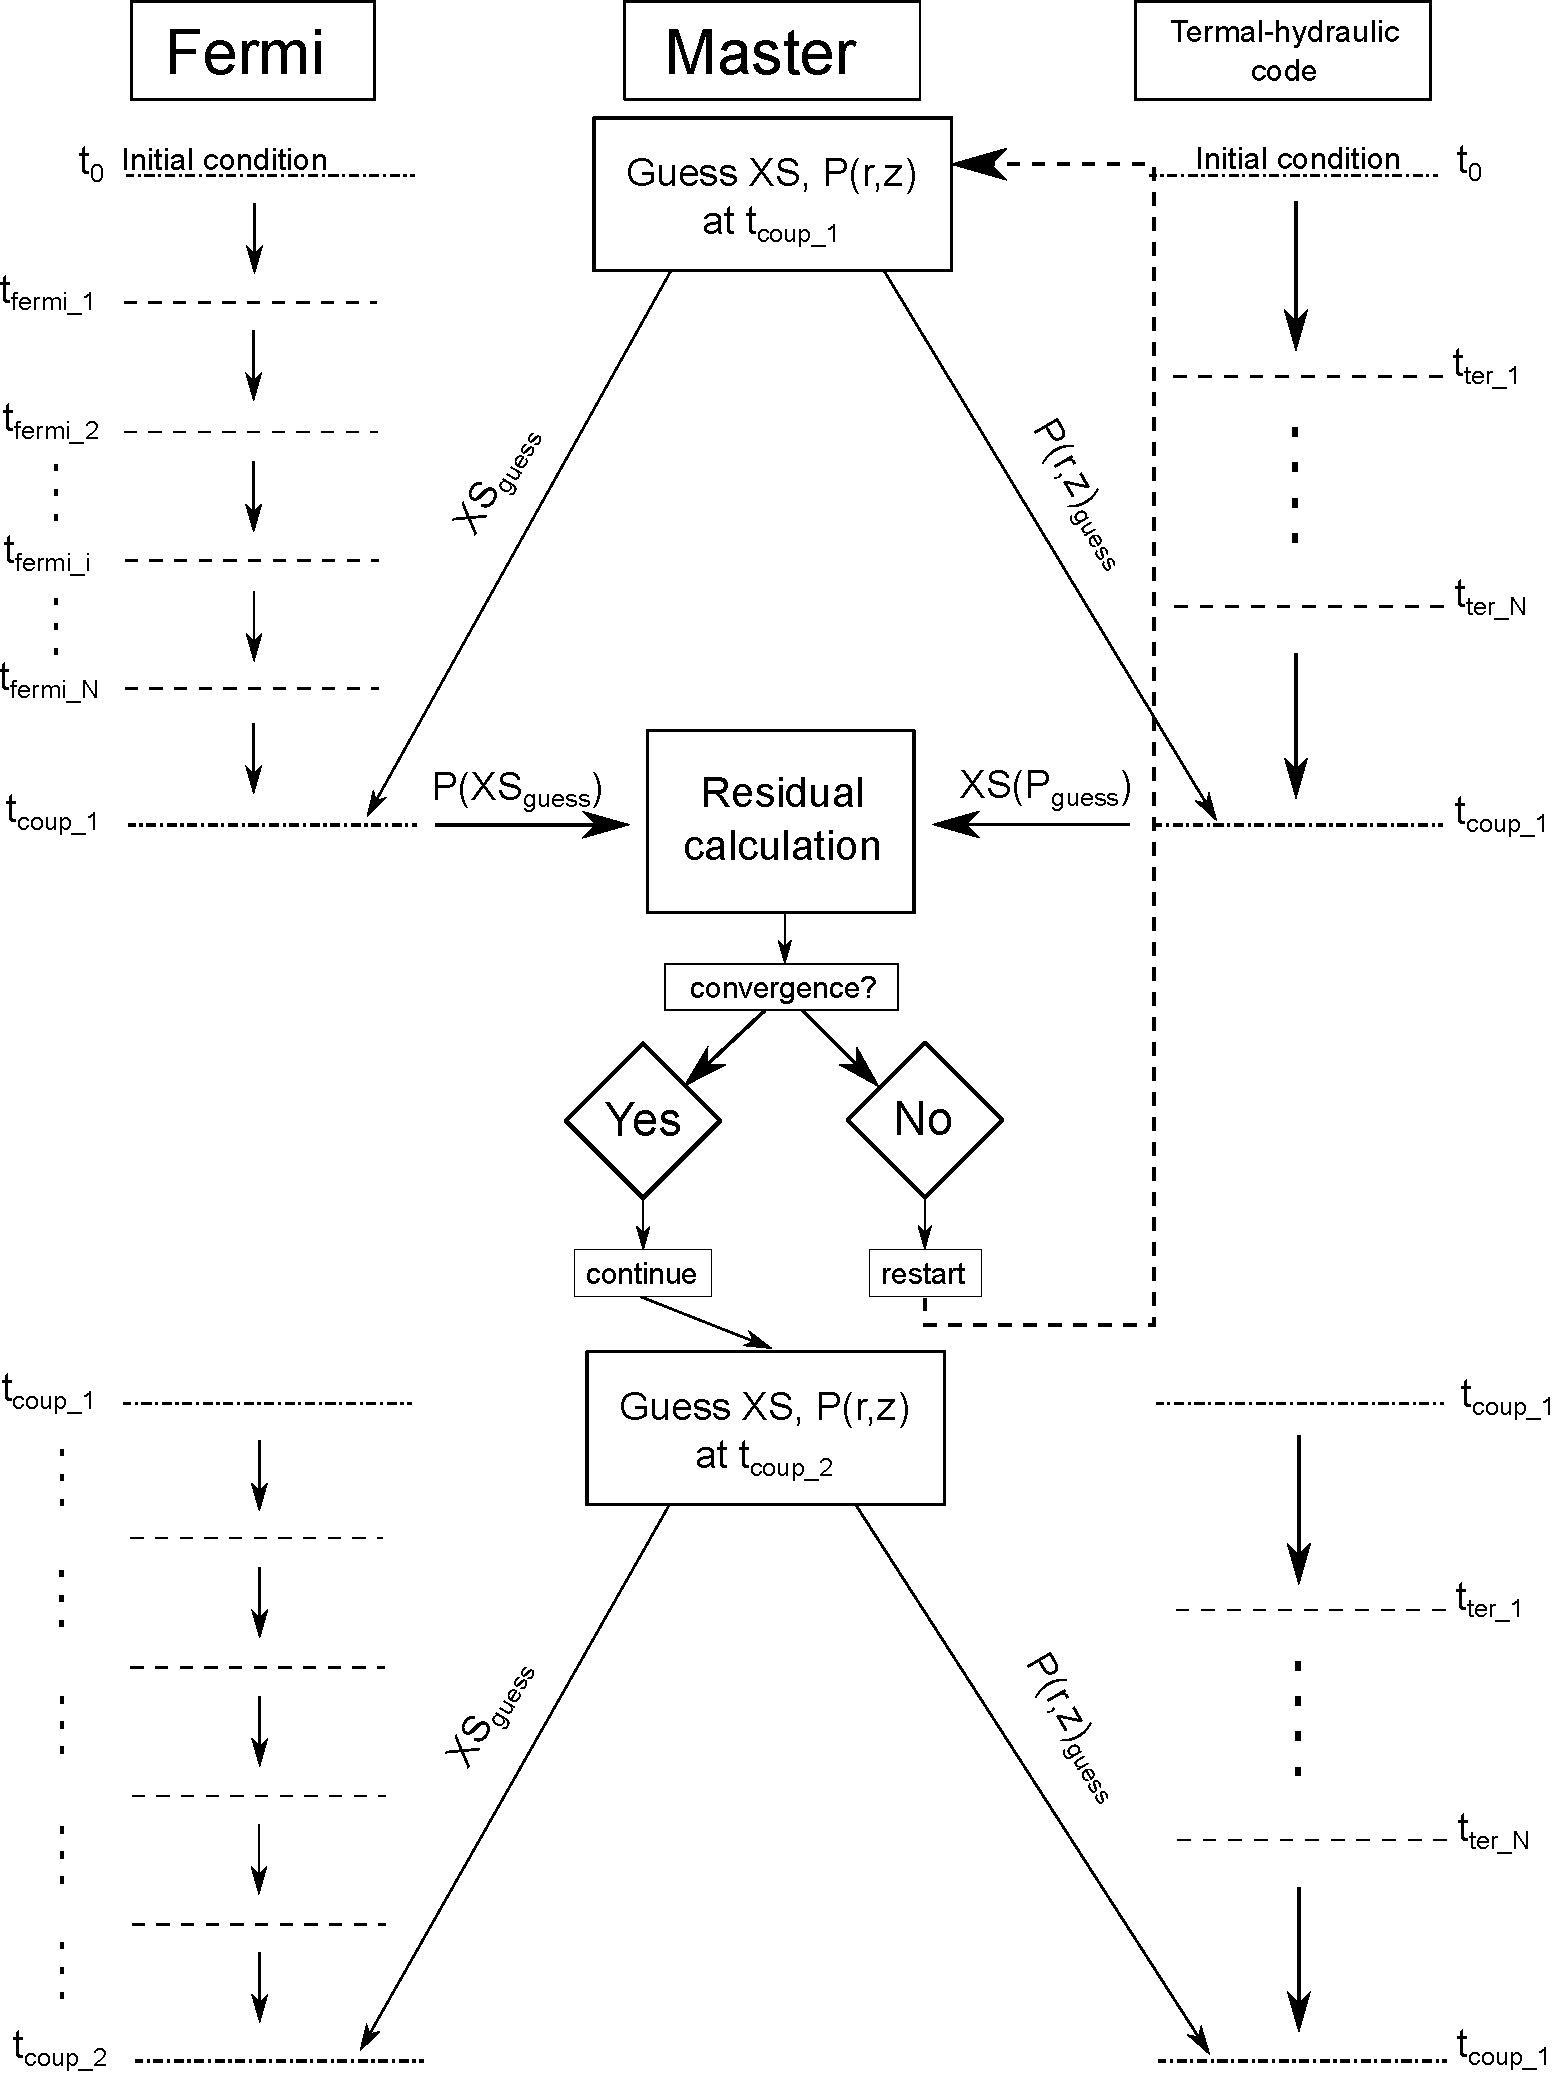
\includegraphics[width=0.55\textwidth]{./images/coupling.pdf}
  \caption{Strategy scheme in evolution calculation using 2 codes coupled by a master code.
    Fermi solves the neutronic equations having as input material corss sections.
    The cross sections received from the master code corresponds at $t_{coup_1}$,
    hence Fermi has to interpolate at each local time step this values with the values of the initial condition.
    Once $t_{fermi}$ reaches $t_{coup_1}$, Fermi sends the calculations to the master code.
    In this example, these calculations are the power spatial distribution.
    At the same time that Fermi was running, a termal-hydraulic code was running too.
    It received power spatial distribution guesses and calculated termal-hydraulic values like temperatures and densities.
    In this example the termal-hydraulic code calculates the cross sections based on this variables.
    The master code computes residuals as the difference between all guesses and calculations.
    If the residuals are nonzeros, which are the common results in the first iterations, the master code has to propose new guesses,
    and both Fermi and termal-hydraulic code have to restart their calculations, starting from back-up solutions at previous $t_{coup}$
    (in the first coupled time step, this solution corresponds to initial conditions).
    When the residuals are zeros, the calculations are strong coupled and each code can continue its evolution, based on guesses at $t_{coup_2}$.
  }
  \label{couplingScheme}
\end{figure}

\section{The master code Newton}
Newton is a code designed to couple another codes that solve particular differential equations.
It has implemented succesfully all necessary functions that corresponds to a master in the coupling strategy described above.
Even when the user can't programm the necessary communication functions in the slave codes,
Newton design allows to easy implement functions that spawn process of the required code,
writing their inputs and reading their outputs,
circumventing the necessity of programming MPI communication functions.
So, for example, Fermi can be coupled in a transitory problem with RELAP,
and both communicates with Newton by different ways:
Fermi communicates via MPI functions and RELAP communicates via input writing and output reading.

Newton ha implemented several numerical methods to solve the residual equations.
To go deeper into Newton, visit https://bitbucket.org/ibnuc/newton/overview.


%%%%%%%%%%%%%%%%%%%%%%%%%%%%%%%%%%%%%%%%%%%%%%%%%%%%%%%
% Sample table                                        %
% Source: www1.maths.leeds.ac.uk/latex/TableHelp1.pdf %
%%%%%%%%%%%%%%%%%%%%%%%%%%%%%%%%%%%%%%%%%%%%%%%%%%%%%%%
% \begin{table}[ht]
% \caption{Sample table} % title of Table
% \centering % used for centering table
% \begin{tabular}{c c c c}
% % centered columns (4 columns)
% \hline\hline %inserts double horizontal lines
% S. No. & Column\#1 & Column\#2 & Column\#3 \\ [0.5ex]
% % inserts table
% %heading
% \hline % inserts single horizontal line
% 1 & 50 & 837 & 970 \\
% 2 & 47 & 877 & 230 \\
% 3 & 31 & 25 & 415 \\
% 4 & 35 & 144 & 2356 \\
% 5 & 45 & 300 & 556 \\ [1ex] % [1ex] adds vertical space
% \hline %inserts single line
% \end{tabular}
% \label{table:nonlin} % is used to refer this table in the text
% \end{table}

% Duis aute irure dolor in reprehenderit in voluptate velit esse cillum dolore eu fugiat nulla pariatur. Excepteur sint occaecat cupidatat non proident, sunt in culpa qui officia deserunt mollit anim id est laborum. \\ Lorem ipsum list:
% \begin{itemize}
% \item Mauris sit amet nulla mi, vitae rutrum ante.
% \item Maecenas quis nulla risus, vel tincidunt ligula.
% \item Nullam ac enim neque, non \emph{dapibus} mauris.
% \end{itemize}
% 
% \noindent Lorem ipsum dolor sit amet, consectetur adipiscing elit. Duis risus ante, auctor et pulvinar non, posuere ac lacus. Praesent egestas nisi id metus rhoncus ac lobortis sem hendrerit. Etiam et sapien eget lectus interdum posuere sit amet ac urna\footnote{Lorem ipsum dolor sit amet, consectetur adipiscing elit. Duis risus ante, auctor et pulvinar non, posuere ac lacus.}:
% 
% \subsection{Lorem ipsum dolor sit amet, consectetur adipiscing elit.}
% Lorem ipsum dolor sit amet, consectetur adipiscing elit. Duis risus ante, auctor et pulvinar non, posuere ac lacus. Praesent egestas nisi id metus rhoncus ac lobortis sem hendrerit. Etiam et sapien eget lectus interdum posuere sit amet ac urna. Aliquam pellentesque imperdiet erat, eget consectetur felis malesuada quis. Pellentesque sollicitudin, odio sed dapibus eleifend, magna sem luctus turpis, id aliquam felis dolor eu diam. Etiam ullamcorper, nunc a accumsan adipiscing, turpis odio bibendum erat, id convallis magna eros nec metus. Sed vel ligula justo, sit amet vestibulum dolor. Sed vitae augue sit amet magna ullamcorper suscipit. Quisque dictum ipsum a sapien egestas facilisis. 
% 
% \subsection{Lorem ipsum dolor sit amet, consectetur adipiscing}
% Lorem ipsum dolor sit amet, consectetur adipiscing elit. Duis risus ante, auctor et pulvinar non, posuere ac lacus. Praesent egestas nisi id metus rhoncus ac lobortis sem hendrerit. Etiam et sapien eget lectus interdum posuere sit amet ac urna. Aliquam pellentesque imperdiet erat, eget consectetur felis malesuada quis. Pellentesque sollicitudin, odio sed dapibus eleifend, magna sem luctus turpis, id aliquam felis dolor eu diam.

\end{document}
